%!TEX root = ../main.tex

\chapter{Preliminary project}

\section{The game engine}

\paragraph{What to choose?:} 
There are three main way to develop on the Meta Quest 2:

\begin{itemize}
  \item \textbf{Native:} By using native \ac{API} that Meta provides for the \ac{HMD}.
  \item \textbf{Unity:} Is a famous game engine principally used for lightweight video games, It is pretty functional and easy to use, its programming language is C\#.
  \item \textbf{Unreal Engine:} Is a famous game engine used for big games, its performance is the best in the market, it uses C++ and a graphical programming language called Blueprint.
\end{itemize}
\noindent
As we said in the non-functional requirements we will use a game engine, I have opted for \ac{UE} because of its performance, the 3D models are pretty complex (\textasciitilde10MByte in size),
so we need good performance.
It has a lot of tools for multiplayer and a nice documentation other than a big community of developers.

\begin{figure}[h]
  \centering
  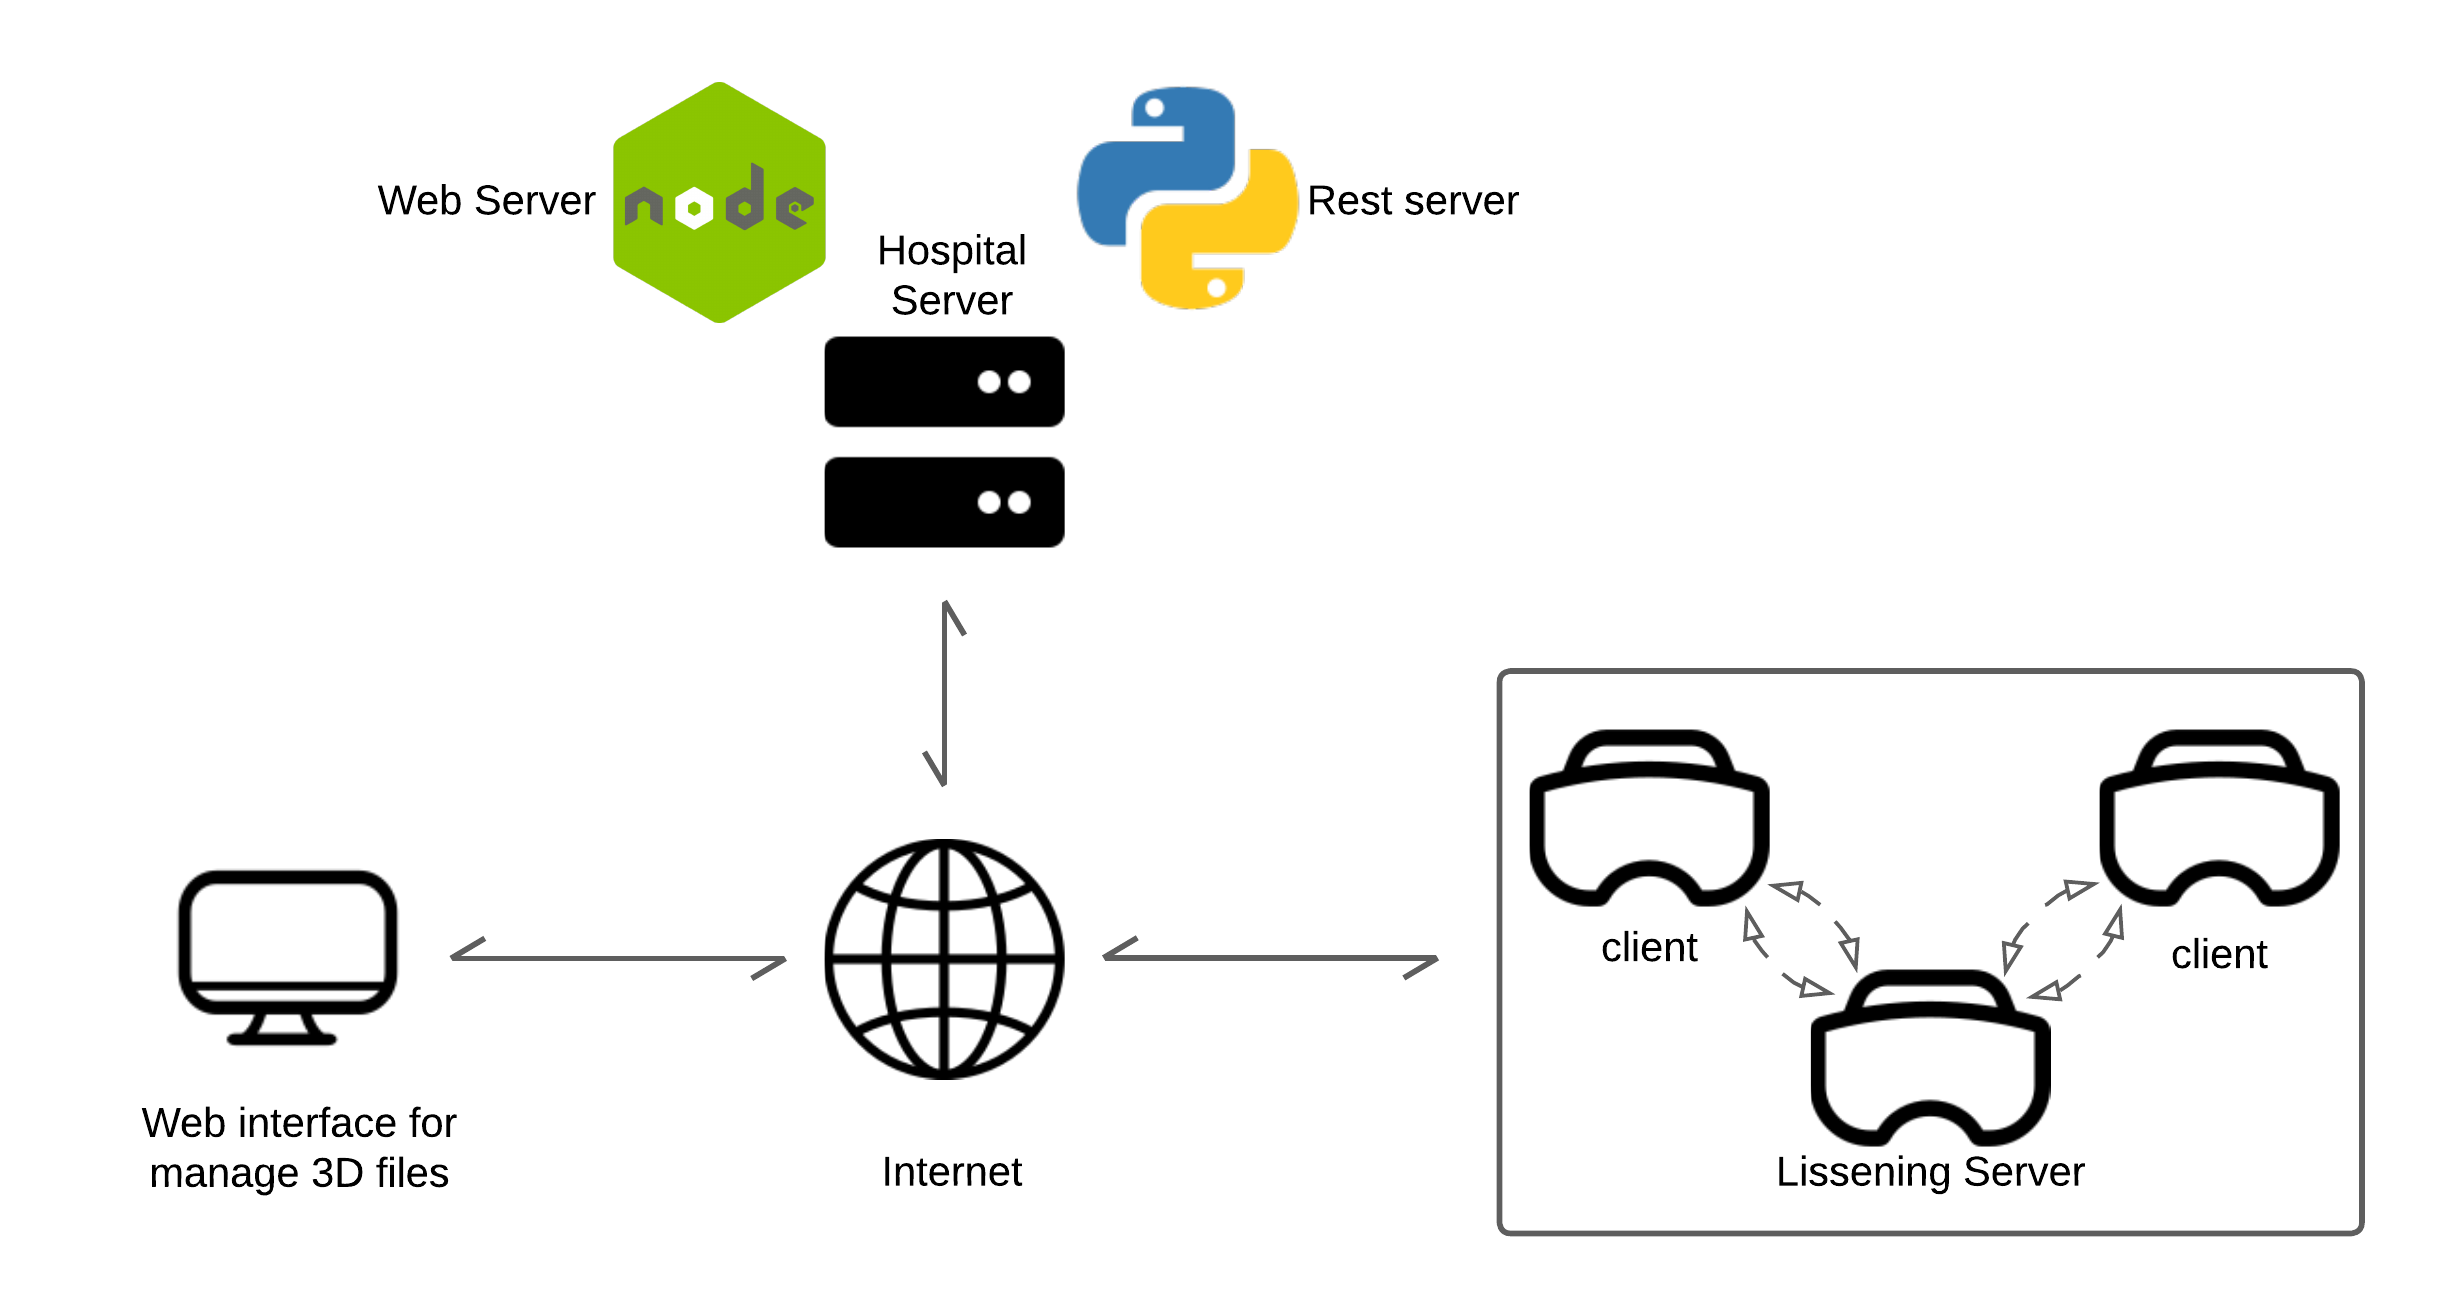
\includegraphics[width=\textwidth]{networkSchema.png}
  \caption{Network Schema}
  \label{fig:NetworkSchema}
\end{figure}